\documentclass[a4paper,11pt]{article}
\usepackage[a4paper,total={18cm, 24cm}]{geometry}
\usepackage[parfill]{parskip}
\usepackage[utf8]{inputenc}
\usepackage[T1]{fontenc}
\usepackage{fancyhdr}
\usepackage[ddmmyyyy]{datetime}
\usepackage{graphicx}
\usepackage{subcaption}
\usepackage{multirow}
\usepackage{hyperref}
\usepackage{amsfonts}

\pagestyle{fancy}
\fancyhf{}
\lhead{\today}
\chead{Deep Learning - Metric Learning}
\rhead{Jakub Rada}

\begin{document}
In this assignment we study image retrieval systems and metric learning.
More specifically, we implement a simple image retrieval system that to a given query images ranks other images based on squred Euclidean distance and outputs the most similar ones.
Then, we compute the Mean Average Precision to evaluate the used loss function and show the precision-recall curve for it.
We start with a pre-trained model with Cross Entropy loss and in the second part we implement two specialized loss functions, the Triplet loss and SmoothAP loss, and train the same network using these losses.
We then compare them with the Cross Entropy loss on the retrieved images and the precision-recall curves.

\section{Retrieval}

\paragraph{Distances} We start by implementing a function to compute pairwise distances between two sets of feature vectors $f^1 \in \mathbb{R}^{N \times D}$ and $f^2 \in \mathbb{R}^{M \times D}$.
We leverage the fact that the features are normalized to have unit length, i.e. $||f^1_{i,:}|| = 1$ and $||f^2_{i,:}|| = 1$.

We will derive it generally for two vectors $x, y \in \mathbb{R}^D$ that have unit norm.
$$
    ||x - y||^2 = (x - y)^T(x - y) = x^Tx - x^Ty - y^Tx + y^Ty = ||x||^2 - 2x^Ty + ||y||^2 = 2 - 2x^Ty
$$
From the derivation we can see that it is sufficient to compute the dot product of the two vectors, which can be done easily using \texttt{einsum(ik,jk->ij, f1, f2)} in PyTorch.

\paragraph{Retrieval} Next, we did the retrieveal of the images using the squared Euclidean distance to rank the images.
The results are shown in Figure \ref{fig:retrieval_ce}, where the green borders have retrieved images with the same label as the label of the query and the red borders mark images with different label.
\begin{figure}[ht]
    \centering
    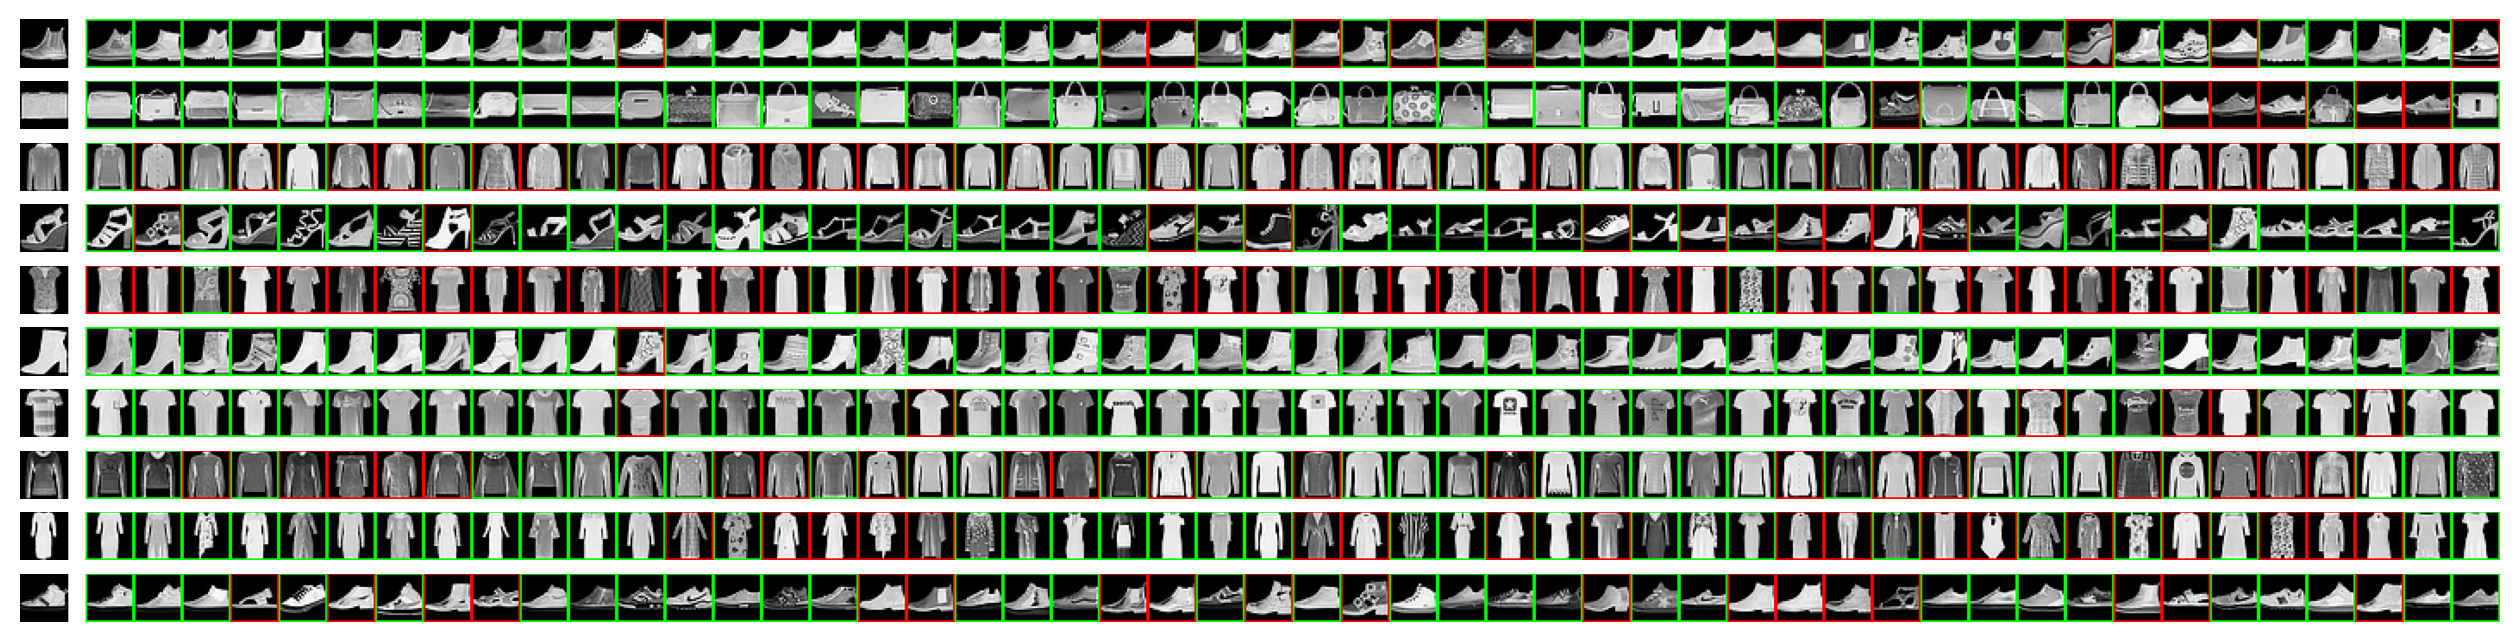
\includegraphics[width=\textwidth]{../outputs/ce_retrieval.png}
    \caption{Images retrieved using the pretrained network using Cross Entropy loss}
    \label{fig:retrieval_ce}
\end{figure}

\paragraph{Precision-Recall curve and mAP score} Last in this part, we compute the Mean Average Precision and show the Precision-Recall curve for this network.
The \textbf{mAP} score is $0.58$, which is the same value as mentioned in the assignment instructions.
The precision-recall curve is shown in Figure \ref{fig:pr_ce}.
\begin{figure}[ht]
    \centering
    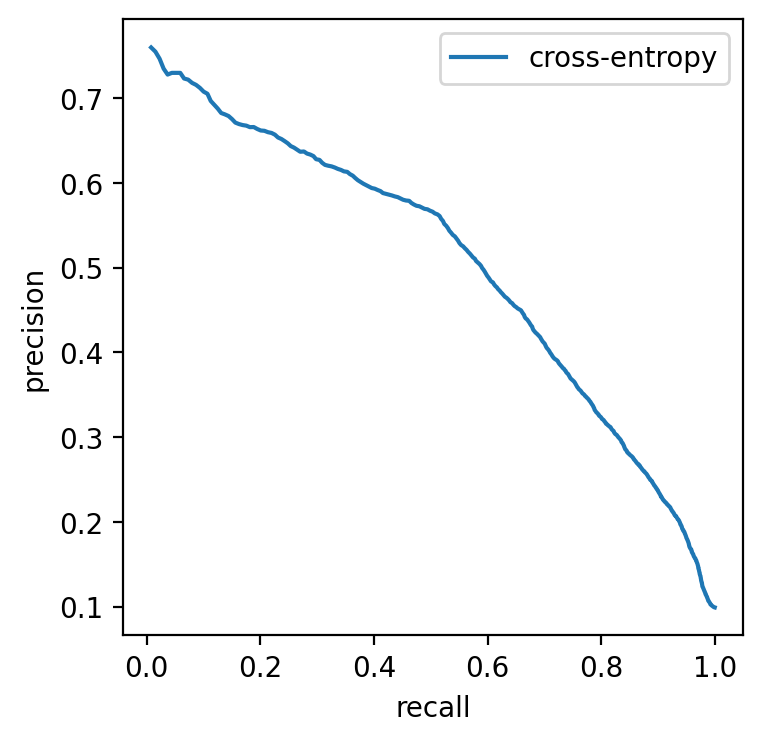
\includegraphics[width=0.5\textwidth]{../outputs/pr_ce.png}
    \caption{Precision-Recall curve for the pretrained network using Cross Entropy loss}
    \label{fig:pr_ce}
\end{figure}

Some of the retrievals are quite interesting.
Some queries have almost all correct retrievals, for example shoes and T-shirts, while others have almost every retrieval wrong, for example jackets and dresses.
I am not sure why that is, maybe the two classes are too similar so the network would need to be trained longer or be bigger to capture more subtle differences.
We will see if the triplet loss or SmoothAP loss can help with this.
The mean average precision is quite low, just slightly above $50\%$, which does not seem that high, even though it is an average across all quries.

\section{Metric Learning}
In previous section, the network was pretrained using the Cross Entropy loss, which is not specifically designed for image retrieval or metric learning.
In this section, we implement two loss functions, which should directly optimize the retrieval performance and we will compare them to see if they indeed perform better.

\paragraph{Triplet loss}
We implemented the triplet loss as described in the assignment instructions and trained the network on the provided data.
From the instructions, it was not clear if we should omit the query image from the positive samples (it is mentioned in computation of \textbf{mAP} but not here), but we decided to omit them.
As suggested, we used first $10$ images as anchors and computed the loss $L_{\mathrm{triplet}}$ as an average of individual losses $l(a)$ for anchor $a$.
We used the margin $\alpha=0.5$ and trained the network for $100$ epochs on random batches of size $64$.
For the triplet loss, I used SGD optimizer with learning rate $0.001$ and no momentum.
The training history is shown in Figure \ref{fig:training_triplet}.

\begin{figure}[ht]
    \centering
    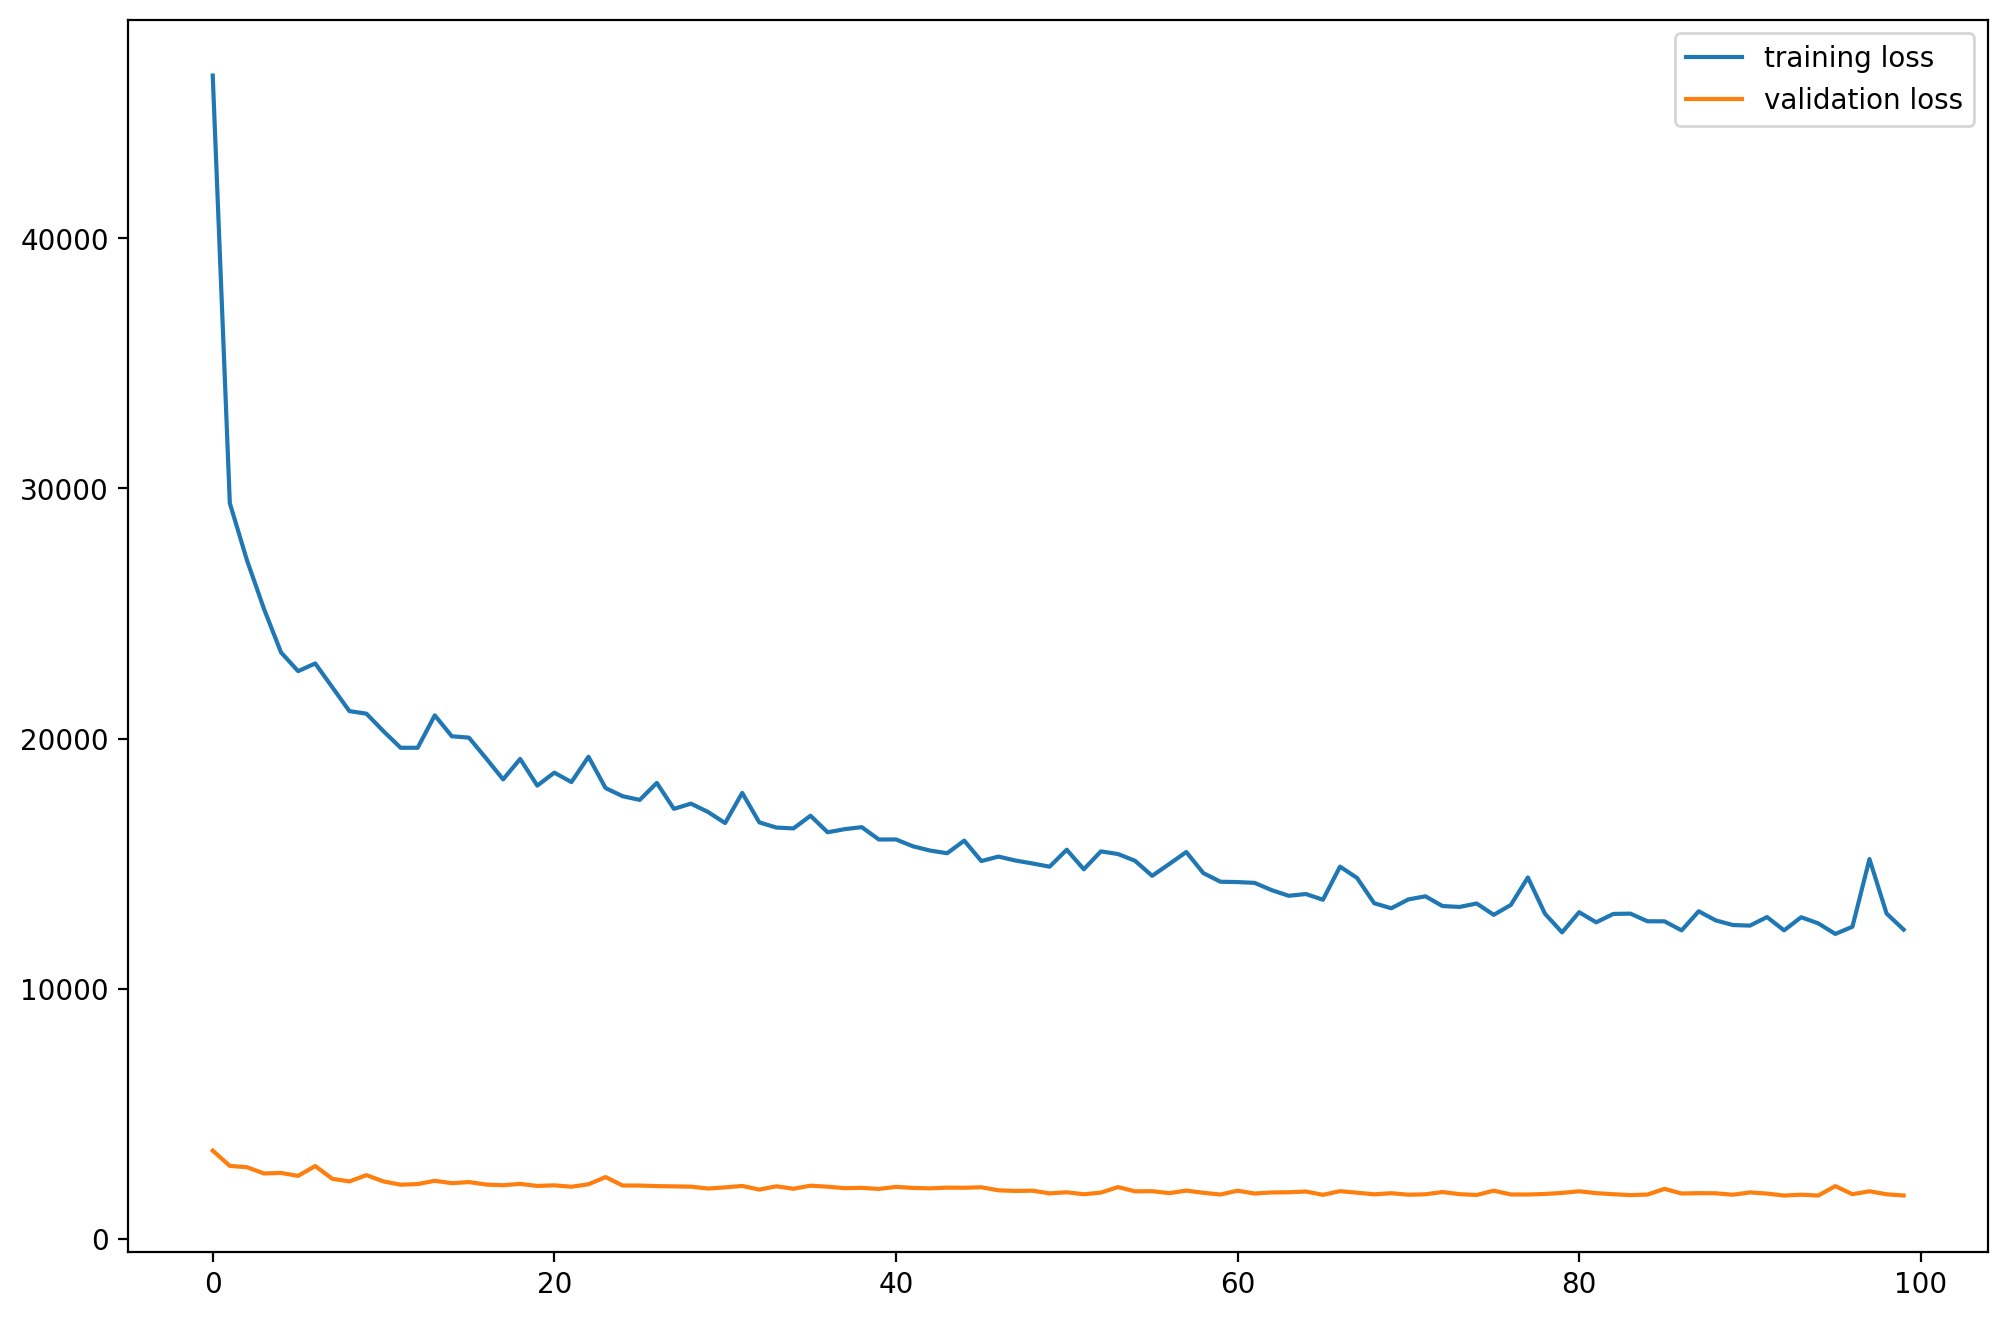
\includegraphics[width=0.5\textwidth]{../outputs/learn_triplet.png}
    \caption{Learning history of the Triplet Loss using SGD with learning rate $0.001$}
    \label{fig:training_triplet}
\end{figure}

From the history plot it looks really well, the loss is decreasing on both the training and validation set.
In contrast to the pre-trained model which used momentum $0.9$, here no momentum was used.
We tried to train the network with momentum as well, but the performance was slightly better without it.
The \textbf{mAP} score is $0.82$ and the retrievals are shown in Figure \ref{fig:retrieval_triplet}

\begin{figure}[ht]
    \centering
    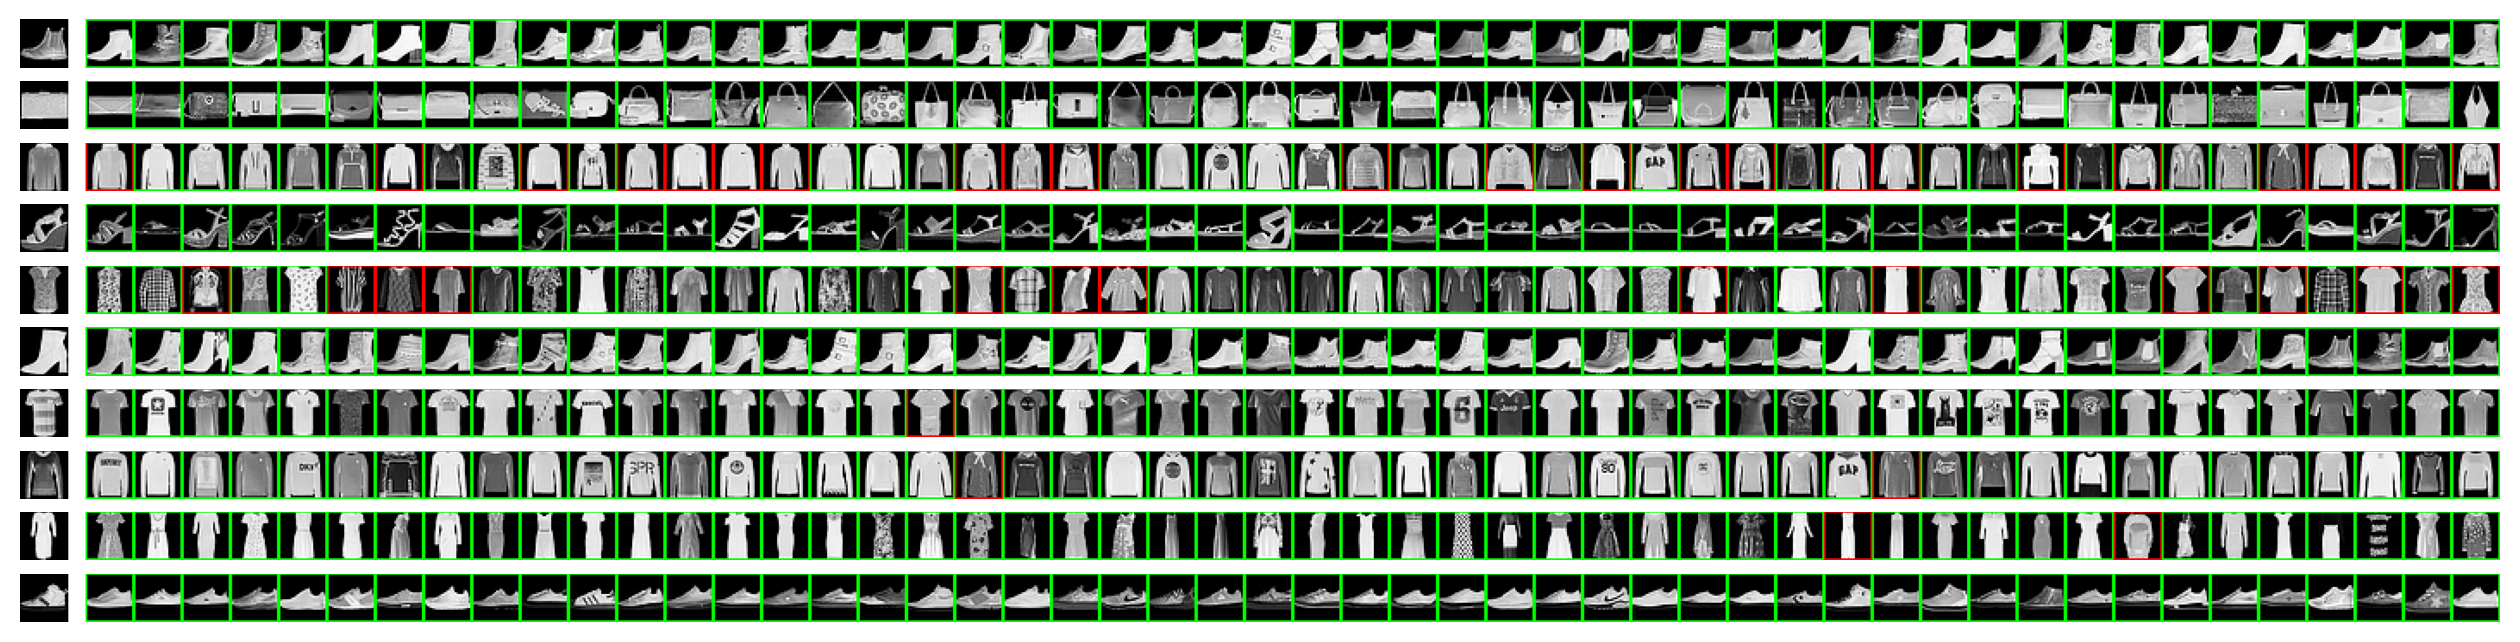
\includegraphics[width=\textwidth]{../outputs/triplet_retrieval.png}
    \caption{Images retrieved using the network trained with Triplet loss}
    \label{fig:retrieval_triplet}
\end{figure}

The retrievals are much better than with the pre-trained network.
There are still some errors but mostly in the jacket row.
The precision-recall curve is shown in Figure \ref{fig:pr} toghether with the pre-trained network and the SmoothAP loss.

\paragraph{SmoothAP loss}
We tried to implement the loss as described on the website but we had troubles optimizing it with SGD.
As with the Triplet loss, used the first $10$ images as anchors and computed the loss $L_{\mathrm{smoothap}}$ as an average of individual losses $l(a)$ for anchor $a$.
I tried two values of $\tau$. $\tau=0.5$ as was in the template and also $\tau=0.01$ as was mentioned in the paper.
The value of $\tau=0.01$ resulted in much better performance.
We trained the network for $100$ epochs.
We tried many different learning rates and momenta but the results were always really bad.
So we looked into the cited paper and made some adjustments to the loss functions.
We have added a normalization by the size of the positive set before the sum so that the criterion looks like this:
$$
    l_{smooth-AP}(a) = \frac{1}{|P|} \sum_{p \in P} \frac{1 + \sum_{n \in N} \sigma_{\tau}(d_p - d_n)}{1 + k_{\sigma}(p)}
$$
Moreover, in the paper they mention that they used the Adam optimizer with learning rate $1e^{-4}$ and weight decay parameter $4e^{-5}$, so we tried this instead and the results were much better as well.
The learning progress can be seen in Figure \ref{fig:training_smoothap}.

\begin{figure}[ht]
    \centering
    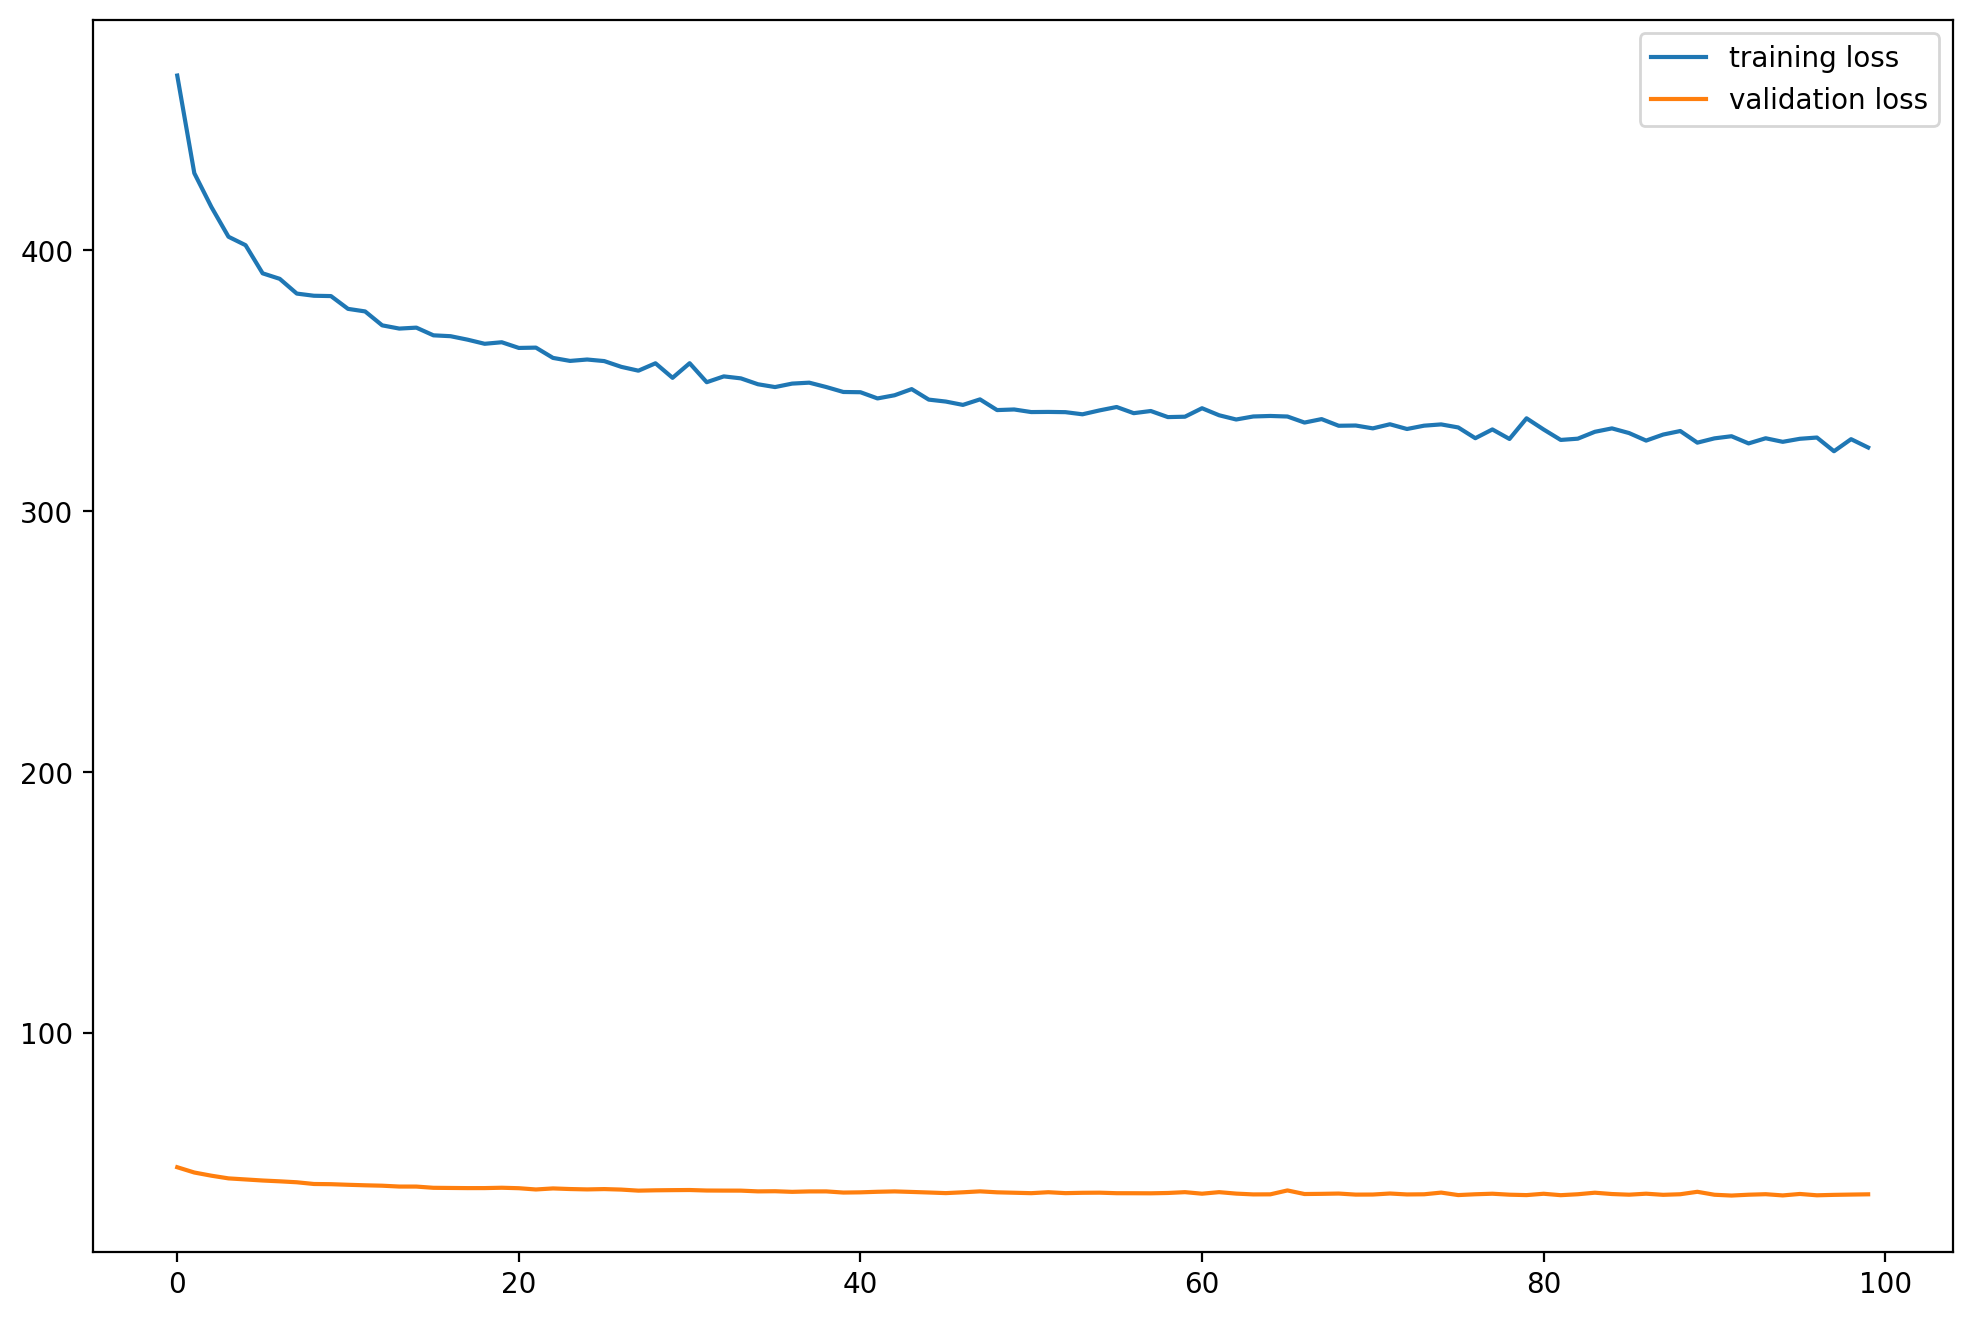
\includegraphics[width=0.5\textwidth]{../outputs/learn_sap.png}
    \caption{Learning history of the SmoothAP loss using Adam with learning rate $1e^{-4}$}
    \label{fig:training_smoothap}
\end{figure}

The learning curve looks also well, the loss is steadily decreasing, maybe not as fast as with the Triplet loss.
That can be caused by the fact that we modified the crieterion to be normalized by the size of the positive set thus making the values of the loss smaller in magnitude.
Performance on the retrieval task on the test set is shown in \ref{fig:retrieval_sap} and the \textbf{mAP} score is $0.8$.

\begin{figure}[ht]
    \centering
    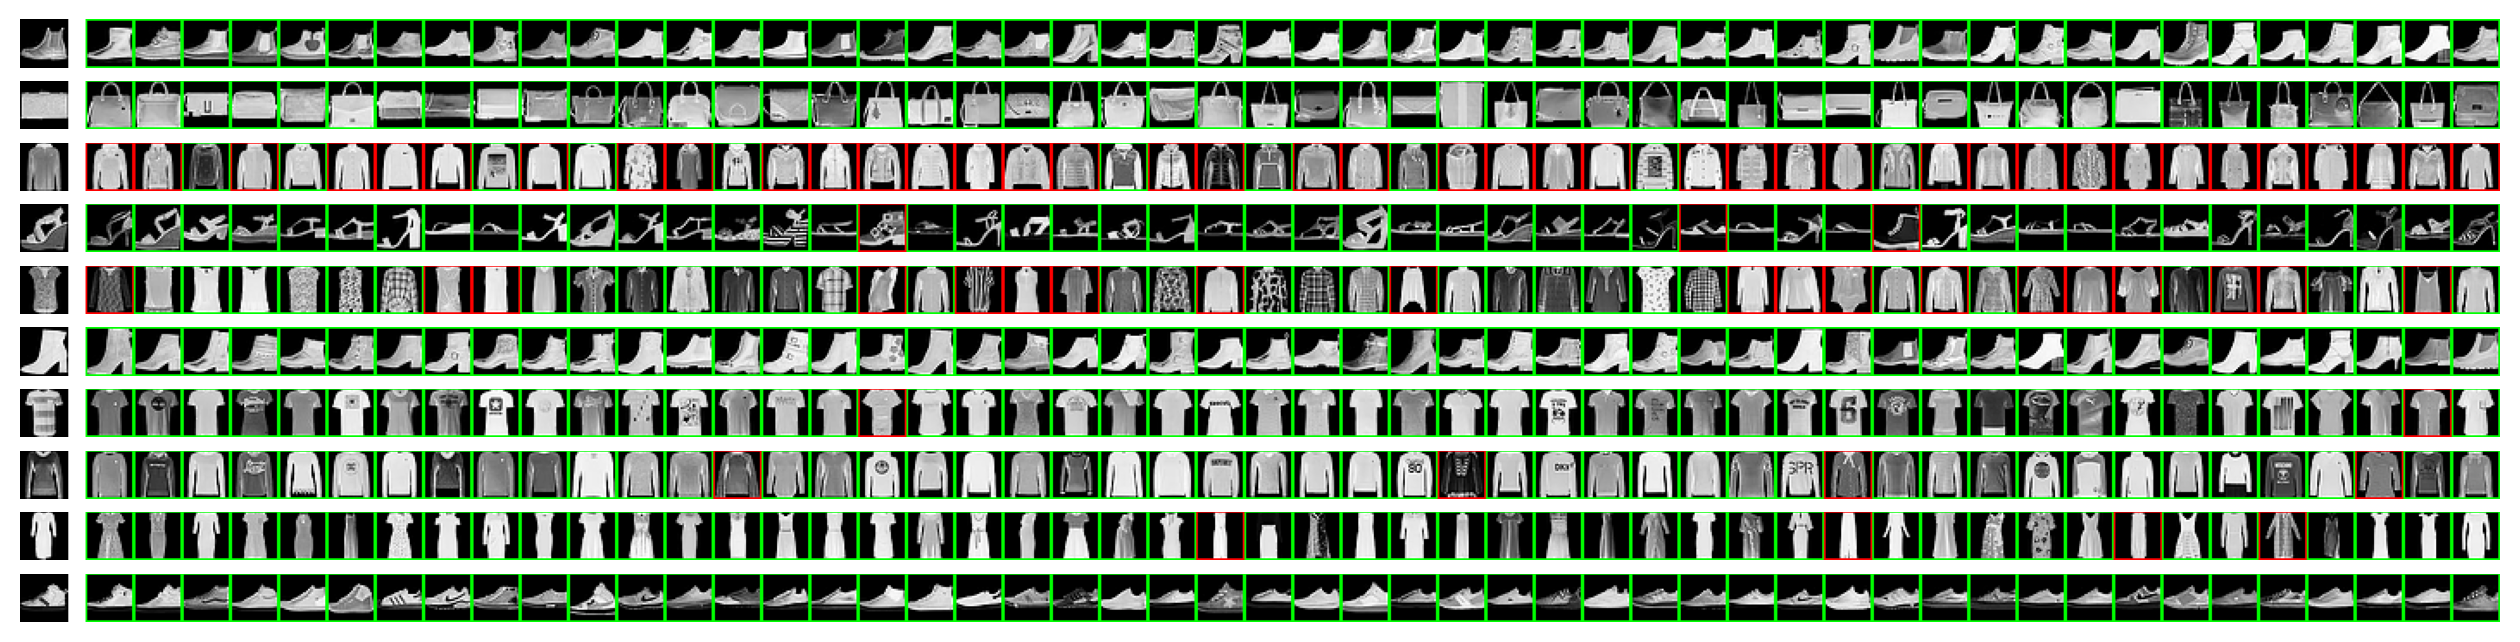
\includegraphics[width=\textwidth]{../outputs/sap_retrieval.png}
    \caption{Images retrieved using the network trained with SmoothAP loss}
    \label{fig:retrieval_sap}
\end{figure}

The retrieval is not as good as with the Triplet loss, the jackets are still causing problems in retrieval.

Finally, we present the precision-recall curves for all three losses in Figure \ref{fig:pr}.
We can see that the Triplet loss is the best, with SmoothAP loss slightly behind.
The cross-entropy loss is clearly not as suitable for this task.

\begin{figure}[ht]
    \centering
    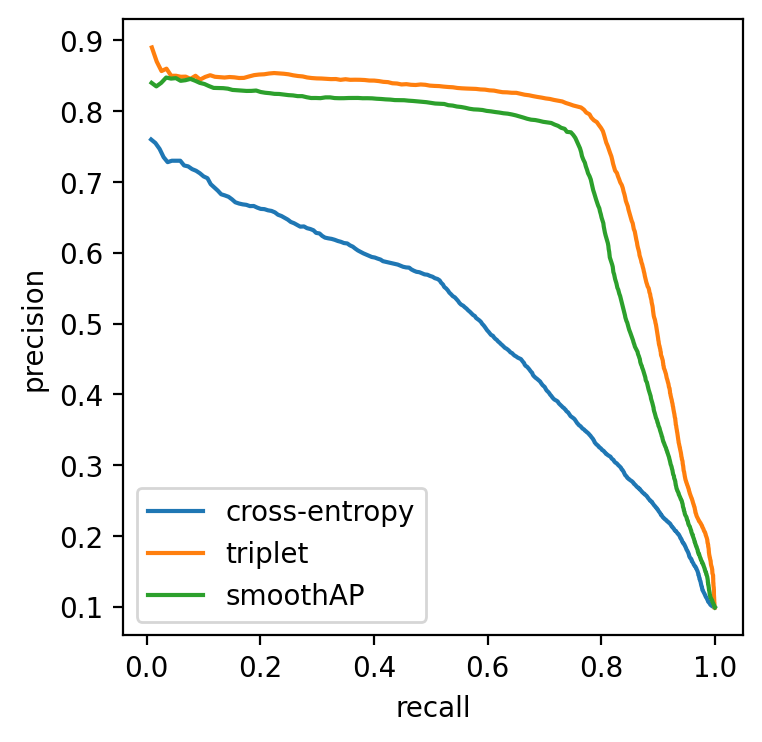
\includegraphics[width=0.5\textwidth]{../outputs/pr.png}
    \caption{Precision-Recall curves for the networks with all three losses}
    \label{fig:pr}
\end{figure}

\section{Discussion}
From the experiments we made, we can conclude that the Triplet loss is clearly better than the Cross Entropy loss.
Even for different settings of the SGD optimizer, the Triplet loss was always learning quite well and reached higher \textbf{mAP} score.
The best performance was achieved with learning rate $0.001$ and no momentum.
For most of the queries, vast majority of the $50$ retrievals were correct only with some errors especially in the jacket query.
Some queries had only positive retrievals.

On the other hand, we had troubles with the SmoothAP loss.
It was hard to optimize with SGD, the best result we achieved was only slightly better than the Cross Entropy loss network.
Maybe we have some error in the implementation, but the losses after an epoch were just oscilating around some value of loss for most learning rates and momenta combinations we tried with only slight decreasing trend.
Thus, we got inspiration from the paper of the authors and slightly modified the loss function to account for the size of the size of the positive set.
Moreover, the authors used the Adam optimizer and some set of parameters mentioned in the text above.
With these adjustments we were able to train the network to achieve comparable performance to the Triplet loss.
In the reference solution, the SmoothAP loss is better but from the learning history plot \ref{fig:training_smoothap} we can see that the loss would most likely decrease still, so with more epochs we would likely overcome the Triplet loss as well.

\end{document}
